\chapter{Introduction}
\label{chapter1}

\section{Background and Motivation}
The Sun, a typical star at the center of our solar system, displays various forms of activity across different scales. This includes energetic eruptive events like solar flares and Coronal Mass Ejections (CMEs), driven by the release of magnetic energy stored in complex magnetic structures in the solar atmosphere \citep{moore_2001, priest_forbes_2007, zhang_2012, amari_2014}. These events release electromagnetic radiation and energetic particles \citep{schwenn_2006, pulkkinen_2007}, affecting \textit{space weather} \citep{schrijver_2010, eastwood_2017} (Fig.~\ref{fig_sw}). They cause disturbances in near-Earth and planetary environments, impacting communication, satellites, power grids, aviation, and space missions \citep{lanzerotti_2001, schwenn_2006, pulkkinen_2007, lilensten_2014}.

Understanding these solar phenomena and their impacts is crucial globally. Research aims to uncover the underlying physical processes through observations, theory, and modeling, while also developing predictive capabilities for space weather. This field, known as \textit{heliophysics} \citep{schrijver_siscoe_2010}, encompasses studying solar, heliospheric, and geospace plasma processes, their impacts on technology and space assets, and strategies for prevention and mitigation \citep{schrijver_2015a, schrijver_2015b}. Initiatives like NASA's Living With a Star program and the National Science Foundation's Space Weather activities drive scientific understanding and predictive capabilities \citep{brewer_2002}.

This thesis focuses on investigating key aspects of solar eruptive activity and its impacts within the realm of heliophysics and space weather. Specific topics include studying the propagation of coronal disturbances triggered by CMEs and flares, the characteristics of solar type III radio bursts, and forecasting Solar Energetic Particle (SEP) events, which pose significant space radiation hazards.

\begin{figure}[!htp]
	\centerline{\includegraphics[width=0.9\columnwidth]{chapter1/figs/srbs.jpeg}}
	\caption{On the left side, a graphical illustration, adapted from ESA/A. Baker, CC BY-SA 3.0 IGO, depicts different eruptive phenomena, while on the right side, there is a representation of spacecraft data (specifically Wind/Waves data from \citet{gopalswamy_2019}) showcasing a radio dynamic spectra, emphasizing distinct spectral categories of SRBs on November 9, 2000. Type-II bursts are correlated with the shock front of a CME, whereas Type-IIIs are connected with the acceleration of SEPs. Image courtesy\protect\footnotemark}
	\label{fig_sw}
\end{figure}

The thesis investigates the origins and propagation mechanisms of transient phenomena resulting from solar eruptions. It employs observational data, analytical theory, modeling, and data science techniques. Despite decades of study using space mission observations, gaps persist in understanding their underlying physics and space weather impacts. The thesis aims to provide new insights within the framework of heliophysics research. Each research topic is explored in dedicated chapters, discussing background, significance, observational challenges, knowledge gaps, and relevant literature. More details can be found in the thesis. 

\footnotetext{\url{https://www.dias.ie/cosmicphysics/astrophysics/astro-surround/}}

\subsection{Coronal Waves}
Coronal waves, also known as Coronal Bright Fronts (CBFs) or EUV waves, are large-scale arc-shaped disturbances observed propagating across the solar corona following the eruption of CMEs and solar flares \citep{thompson_1998, nindos_2008, vrsnak_2008, magdalenic_2010, veronig_2010, warmuth_2015}. These waves, visible in EUV, white-light coronal emission, and radio wavelengths, can span distances of up to several hundred Mm and travel at speeds ranging between 100-1000 \kms, faster than the local characteristic speed in the corona, eventually transforming into shock waves \citep{pick_2006, thompson_2009, nitta_2013, liu_2014}. They consist of piled-up plasma with higher density, making them appear brighter in white-light images.

Discovered through observations obtained with the Extreme ultraviolet Imaging Telescope (EIT) instrument on the Solar and Heliospheric Observatory (SOHO) that was launched in 1995, coronal waves appear as bright propagating fronts in 19.5 nm wavelength imaging of Fe XII emission lines formed at approximately 1.5 MK plasma \citep{thompson_1998}. Subsequent studies using SOHO/EIT and the Transition Region and Coronal Explorer (TRACE) found correlations between coronal waves and CMEs, suggesting they are fast-mode magnetohydrodynamic (MHD) waves driven by CME lateral expansions \citep{biesecker_2002}.

Since 2010, the initiation and evolution of coronal waves have been observed with unprecedented resolution by the Atmospheric Imaging Assembly (AIA) on the Solar Dynamics Observatory (SDO), using multiple EUV passbands sensitive to a wide temperature range \citep{lemen_2012, nitta_2013}. Observing and studying coronal shock waves remotely is typically done through EUV observations using space-based instruments like AIA onboard the SDO spacecraft. Alternatively, shock waves can be indirectly observed through the detection of type II radio bursts, commonly associated with shock waves in the solar corona \citep{vrsnak_2008}.

The AIA instrument, with its exceptional spatial and temporal resolution, has provided significant insights into the dynamics of the low solar corona over the past decade \citep{patsourakos_2010, ma_2011, kozarev_2011}. By observing the solar disk in bands 193 and 211 $\AA$, it distinguishes compressive waves in the lower corona, offering valuable information about the kinematics and geometric structure of CBFs. Observations off the solar limb are preferred to study the evolution of the wave's leading front accurately, mitigating projection effects that may introduce ambiguities \citep{kozarev_2015}.

CMEs typically consist of three parts (Fig.~\ref{fig_cme}): the CME Front, CME Cavity, and CME Core \citep{vourlidas_2013}. CBFs form in front of the expanding front of CMEs. In situ observations of shock waves classify them into quasi-parallel, quasi-perpendicular, sub-critical, and super-critical shocks based on the angle between the wavefront normal vector and the upstream magnetic field lines \citep{tsurutani_1985}. Coronal waves display diverse morphology and kinematics, ranging from circular fronts to narrow jets or expanding dome-like structures \citep{veronig_2010}. However, fundamental questions persist regarding their physical nature and drivers \citep{chen_2016, vrsnak_2008, warmuth_2015}, including whether they are true wave disturbances or pseudo-wave fronts \citep{wills_2007, vrsnak_2008, delannee_1999, chen_2002}.

\begin{figure}[!htp]
	\centerline{\includegraphics[width=0.8\columnwidth]{chapter1/figs/AIA_LASCO_composite_2022613.png}}
	\caption{Composite image from the AIA and LASCO telescopes on the NASA-GSFC SDO and NASA/ESA SOHO spacecrafts shows a large CME being ejected to the east and its typical structure.}
	\label{fig_cme}
\end{figure}

Extensive observational and modeling studies have been conducted to evaluate these paradigms, but a consensus remains elusive \citep{patsourakos_2012, long_2017}. Addressing these outstanding questions is crucial, as coronal waves are being incorporated into models as primary agents producing SEP events and geomagnetic storms following CMEs \citep{rouillard_2012, park_2013}. The present thesis undertakes an extensive statistical analysis of coronal EUV wave events observed by SDO to provide new insights into their kinematical properties and relationship to CMEs and plasma properties in the corona. It focuses on analyzing their large-scale evolution as a function of distance and direction from the source region, aiming to uncover systematic trends in their propagation kinematics and exploring relationships between different pairs of kinematical parameters compared to previous works. These results have important implications for incorporating coronal waves into predictive models of CMEs and SEP events for future space weather forecasting.

\subsection{Solar Radio Bursts}
Solar radio emissions, including solar radio bursts, are extensively studied due to their association with solar activity and potential impacts on Earth's atmosphere and technology. Type III bursts, originating from transient energetic electron beams injected into the corona, serve as remote diagnostics for studying energetic electrons and plasma dynamics \citep{ergun_1998, pick_2006, reid_2020}. These bursts, linked to plasma density, offer insights into processes driving solar active phenomena like CMEs and flares \citep{reid_2014, kontar_2017}. They provide valuable information on electron acceleration and transport, shedding light on the dynamic interaction between non-thermal electron distributions and ambient plasma \citep{melrose_1980}.

Pioneering observations in the 1940s led to the classification and subsequent spectrographic studies of solar radio bursts, uncovering emission mechanisms and particle diagnostics \citep{wild_1963, suzuki_1985}. Magnetic reconnection models provided theoretical explanations for particle acceleration generating these bursts \citep{holman_2011}. Radio imaging spectroscopy enables tracking of radio sources on the Sun, offering insights into energetic particle transport from the Sun to Earth \citep{krucker_2011, klassen_2003a, klassen_2003b}. Different burst types are observed and classified based on their spectral characteristics (Fig.~\ref{fig_srb_types}) \citep{wild_1963}, with this thesis focusing on a detailed analysis of solar type III radio bursts.

\begin{figure}[!htp]
	\centering
	\includegraphics[width=0.8\columnwidth]{chapter1/figs/typefignew.png}
	\caption[Classification of solar radio bursts]{Diagram illustrating the classification of solar radio bursts. Image courtesy\protect\footnotemark}
	\label{fig_srb_types}
\end{figure}

Type III bursts manifest as intense enhancements of radio flux with rapid frequency drifts, observable across a broad frequency spectrum from GHz to kHz \citep{wild_1950a, lecacheux_1989, bonnin_2008}. They arise from energetic electron beams ejected during magnetic reconnection, with the rapid drift corresponding to the beams' propagation from the Sun's lower corona outward along open magnetic field lines \citep{cane_2002, macdowall_2003}. Investigating their source locations, plasma environments, and beam kinematics is vital for understanding coronal particle acceleration and transport relevant to SEP forecasting models.

Despite over 50 years of study, gaps persist in understanding the exciter beams and emission mechanisms of type III bursts, including detailed electron acceleration sites, beam configurations, burst onset drivers, and the role of density fluctuations in beam propagation \citep{reid_2018a, reid_2018b, li_2012a}. Recent work combining imaging and spectral data with modeling aims to constrain radio burst exciters in detail \citep{chen_2013b, kontar_2017}, yet challenges remain in reconciling models with observations and predicting radio diagnostics. Coordinated observations and modeling efforts can advance knowledge in these areas, aiding predictions of energetic electron properties based on radio diagnostics. This thesis undertakes a detailed investigation of a solar type III burst, deriving electron beam trajectories, coronal densities, and emission sources, providing insights into the corona plasma environment and energetic electron transport relevant to SEP forecasting applications.

\footnotetext{Types of solar radio bursts: \url{http://solar.physics.montana.edu/takeda/radio_burst/srb.html}}

\subsection{Solar Energetic Protons Forecasting}
Solar energetic protons (SEPs) are high-energy particles originating from solar flares and CMEs, characterized by their high energy levels (up to the GeV/nucleon range) and potential to cause radiation damage \citep{aschwanden_2002, lin_2005, reames_2013}. Their fluence and energy spectrum depend on various factors, including solar activity strength and interplanetary conditions \citep{kahler_1984, kahler_1987, debrunner_1988, miteva_2013, trottet_2015, dierckxsens_2015, le_2017, gopalswamy_2017}. SEPs exhibit a strong association with the solar cycle, peaking during its maximum phase \citep{reames_2013}, although the exact relationship remains complex and not fully understood \citep{nymmik_2007, ramstad_2018}.

Figure~\ref{fig_lasco_sep} illustrates the impact of SEPs during the \textit{Halloween storm} of 2003, a significant solar event. SEPs play a crucial role in adverse space weather, posing radiation hazards to humans and equipment in space \citep{reames_1999}. SEP events consist primarily of protons accelerated by CME-driven shock waves, with gradual events involving protons above \almost10 MeV and impulsive events dominated by electrons and ions like $^3$He \citep{reames_2013, nitta_2015}.

\begin{figure}[!htp]
	\centerline{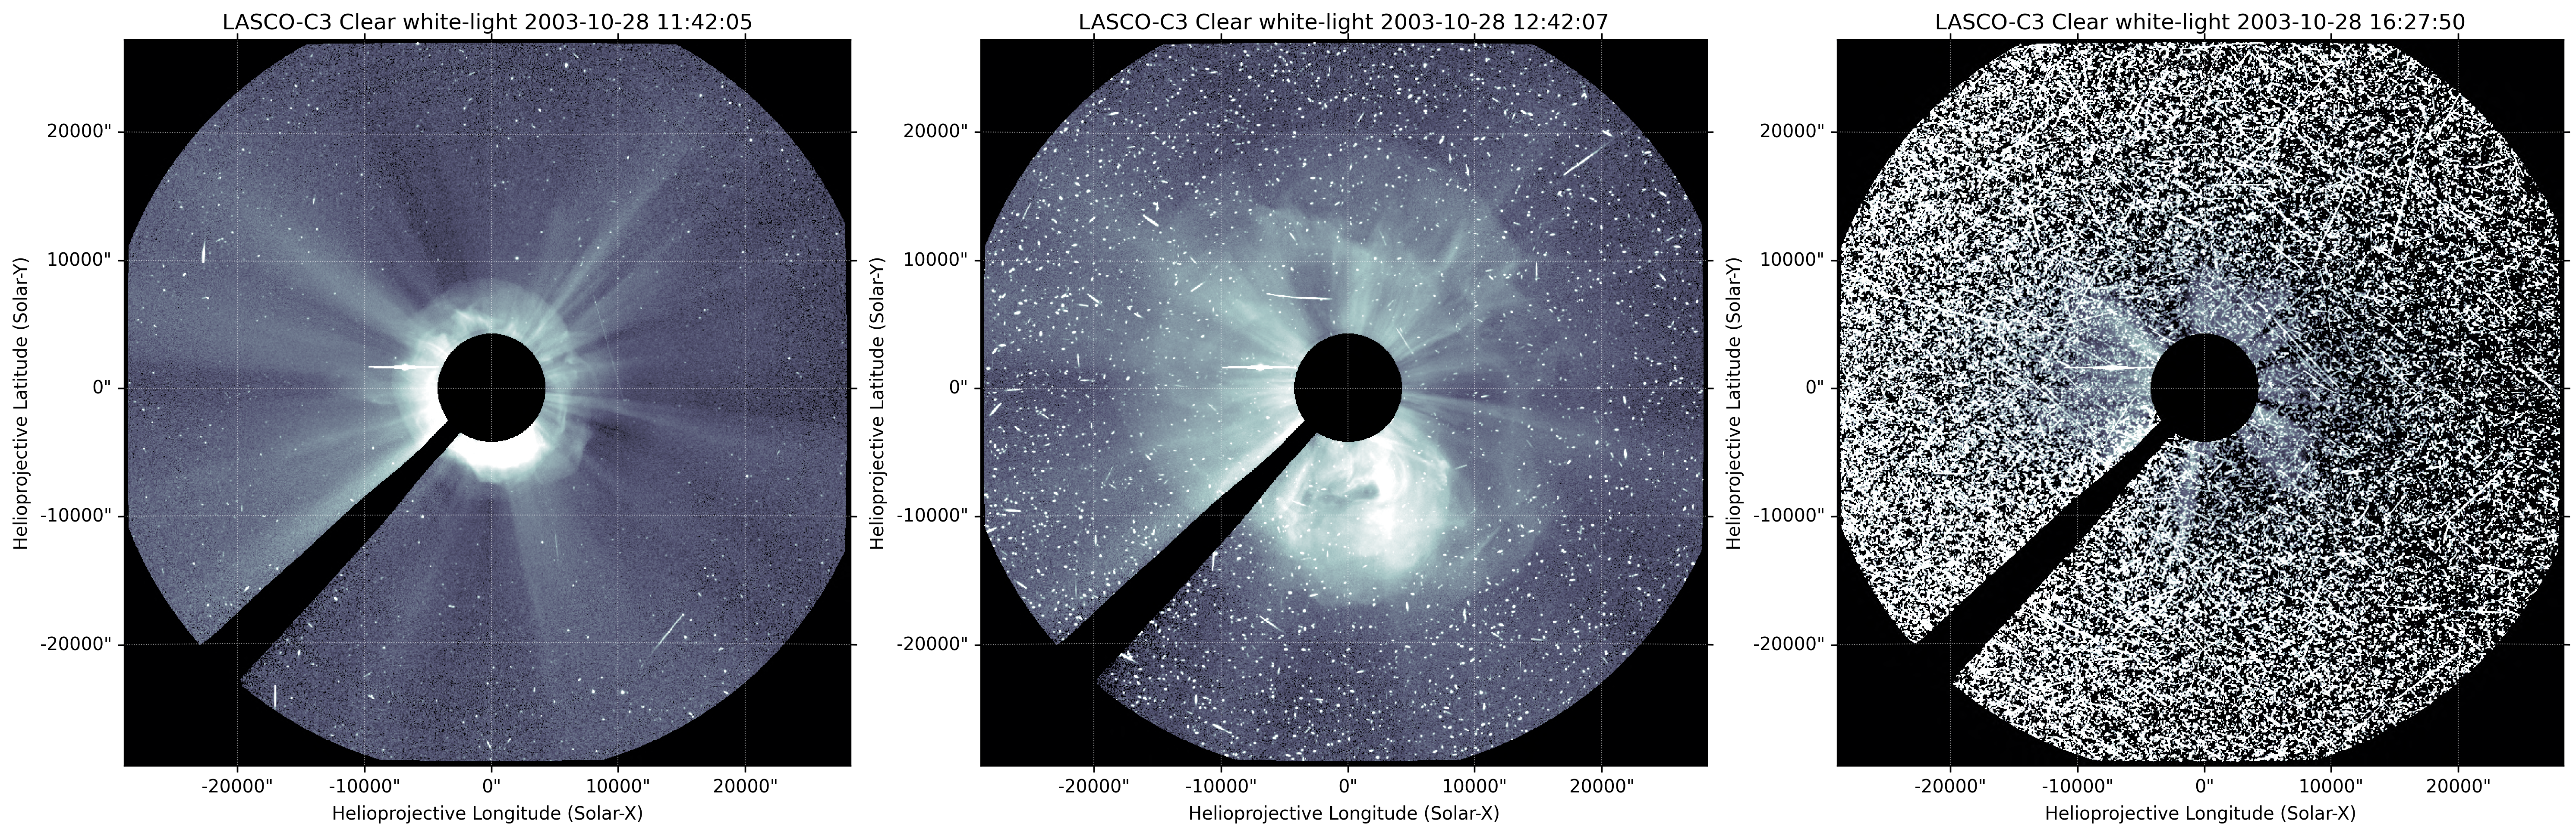
\includegraphics[width=1\columnwidth]{chapter1/figs/LASCO_C3_SEP.png}}
	\caption{Coronagraph image captured by the SOHO/LASCO C3 instrument during a Halo-CME event. The speckled appearance of the corona results from signal contamination due to particles generated when SEPs interact with the SOHO telescope.}
	\label{fig_lasco_sep}
\end{figure}

SEP forecasting models face challenges due to the complex physics involved, motivating the exploration of data-driven approaches using machine learning \citep{kahler_2007, laitinen_2017}. Deep learning techniques offer promising avenues for improved predictions, capturing complex relationships between parameters \citep{florios_2018, camporeale_2019}. This thesis aims to develop deep Neural Network models for predicting SEP intensity profiles, leveraging historical data to enhance forecasting capabilities.

\section{Objectives and Scope}
This PhD thesis explores various solar phenomena, including CBFs, type III radio bursts, and SEP events, aiming to deepen our understanding of solar corona physics and its relation to eruptions and energetic particle radiation.

For CBFs, the research analyzes 26 historical events observed by the AIA instrument on SDO from 2010 to 2017, examining their properties and kinematics in relation to the coronal plasma environment. Techniques like base-difference images and geometric models are employed to derive measurements, alongside exploring shock properties within the CBFs.

The study of type III radio bursts focuses on unraveling their generation mechanisms, identifying their sources in the solar corona, and investigating relationships with magnetic field structures and plasma environment. It analyzes specific bursts observed on April 3, 2019, using data from LOFAR and PSP instruments, comparing observations with existing models and exploring potential burst sources.

In SEP forecasting, the aim is to develop a BiLSTM neural network model capable of predicting daily SEP integral flux over a three-day window for energy ranges $>$10 MeV, $>$30 MeV, and $>$60 MeV. The model's performance is evaluated against established forecasting models using historical SEP data from the past four solar cycles, assessing accuracy and effectiveness through various metrics and correlation analysis.

By addressing these aspects of solar activity, this research advances our understanding of solar dynamics and enhances our ability to predict space weather events impacting Earth.

\section{Outlines}
This dissertation examines CBFs, solar radio bursts, and SEP events. It analyzes the kinematics of CBFs in the solar corona, investigating 26 CBFs associated with SEP events observed between 2010 and 2017. The study employs the SPREAdFAST framework to understand CBF kinematics and plasma parameters, aiding space weather forecasting and SEP event studies (Chapter~\ref{chapter2}). Additionally, it presents a method for identifying and tracking CME-driven shock waves using wavelet transform and image filtering, with applications in deep-learning solar datasets.

Another study in Chapter~\ref{chapter2} explores the correlation between geomagnetic storm intensity and solar and interplanetary phenomena, emphasizing the importance of considering CME speed and magnetic structure orientation for accurate storm prediction. Chapter~\ref{chapter3} focuses on type III radio bursts, analyzing an event on April 3, 2019, and characterizing 16 bursts using multi-wavelength data and models, revealing insights about plasma conditions along burst trajectories.

Chapter~\ref{chapter4} investigates SEP events, modeling their acceleration and transport during coronal shock events through the SPREAdFAST framework, and developing SEP forecasting models using a BiLSTM neural network. The effectiveness of these models is validated through testing and benchmarking against existing ones. Finally, Chapter~\ref{chapter5} summarizes the dissertation's key findings.